% !TEX encoding = IsoLatin

\documentclass{report}
\usepackage[usenames,dvipsnames]{color}
%pour le code
\usepackage{listings}

\usepackage[utf8]{inputenc}
 \usepackage{lmodern}
\usepackage{listings}
\lstset{language=C}
 
 %pour les couleurs !!
 \usepackage[usenames,dvipsnames]{color}

\usepackage{geometry}
\geometry{scale=0.8, nohead}
\usepackage{t1enc}
\usepackage[french]{babel}

\usepackage{url}


 %pour les images
\usepackage{graphicx}
\definecolor{vert}{rgb}{0.2,0.6,0.4} 
\lstset{language=c, breaklines=true, basicstyle=\ttfamily,basicstyle=\scriptsize, keywordstyle=\color{blue}, commentstyle=\color{vert}, stringstyle=\color{red}, identifierstyle=\ttfamily}


\makeatletter

\geometry{ hmargin=2cm, vmargin=2cm}


\makeatletter

\geometry{ hmargin=2cm, vmargin=2cm}

\def\blurb{%
BE Validation de modèles de procédé}


\def\ligne#1{%
  \hbox to \hsize{%
    \vbox{\centering #1}}}%

\makeatletter
\def\maketitle{%
	\null
	\vfill
	\vbox{\centering \Large \textbf{\blurb}}
	\vspace{15mm}
	\vbox{\centering \LARGE \textbf{\@title}}
	\vspace{15mm}
	\vbox{\centering \@author}
	\vspace{8mm}
	\vbox{\centering \@date}
	\vspace{15mm}
	\vbox{\centering \textbf{Résumé du projet}}
	\vspace{5mm}
	\vbox{%
		\setlength{\fboxsep}{10pt}
		\centering \fbox{%
		\begin{minipage}{0.9\textwidth}
			\setlength{\parindent}{1cm}
			\setlength{\parskip}{2ex plus .4ex minus .4ex}                        
			L’objectif de ce mini-projet est de compléter le travail fait en BE IDM et de produire une
                        chaîne de vérification de modèles de processus SimplePDL en utilisant les outils de modelchecking
                        disponibles dans la boîte à outils Tina.
		\end{minipage}%
	}
%
	}
	\vfill
	\clearpage
}

\title{Rapport BE IDM 2012}
\author{
Alexandre Escudero \texttt{<escudero@etud.insa-toulouse.fr>}\\
Mathieu Othacéhé \texttt{<othacehe@etud.insa-toulouse.fr>}}
\date{5ème année SEC}

\begin{document}

\maketitle
\tableofcontents


\nocite{*}

\chapter{Introduction}

\chapter{Partie 1}

\section{T1}

Il s'agit dans cette première section de prendre en compte les ressources et le temps dans le métamodèle.
On reprend donc le fichier SimplePDL.ecore, et l'on ajoute de nouveaux éléments.

\subsection{Ajout des ressources}

Pour la gestion des ressources :\\

On rajoute deux nouvelles classes : RessourceDefinition et RessourceInstance.
La classe RessourceDefinition sert à définir les différentes ressources et leur nombre. Par exemple, si l'on dispose de 4 ressources de type Machine,
on va alors déclarer dans le fichier modèle simplepdl une RessourceDefinition, avec un attribut number égal à 4.\\

La classe RessourceInstance permet d'exprimer le fait qu'une activité va devoir utiliser une certaine quantité de ressources pour fonctionner.
Elle possède un lien vers une RessourceDefinition exprimant le type de la ressource ainsi qu'un lien vers l'activité en question.
Elle doit aussi posséder un attribut entier indiquant le nombre de ressources nécéssaires à l'activité.\\

Si l'on affiche le métamodèle sous forme textuelle (améliorée), on a donc :\\

\begin{figure}[!h] 
\begin{center}
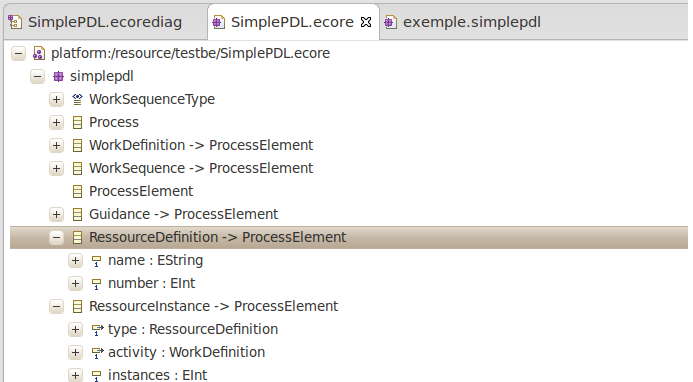
\includegraphics[width=10cm]{Capture-2.png}
\caption{Fichier Ecore modifié} 
\label{img1} 
\end{center}
\end{figure} 

On peut également afficher le métamodèle sous forme graphique Ecorediag :\\

\begin{figure}[!h] 
\begin{center}
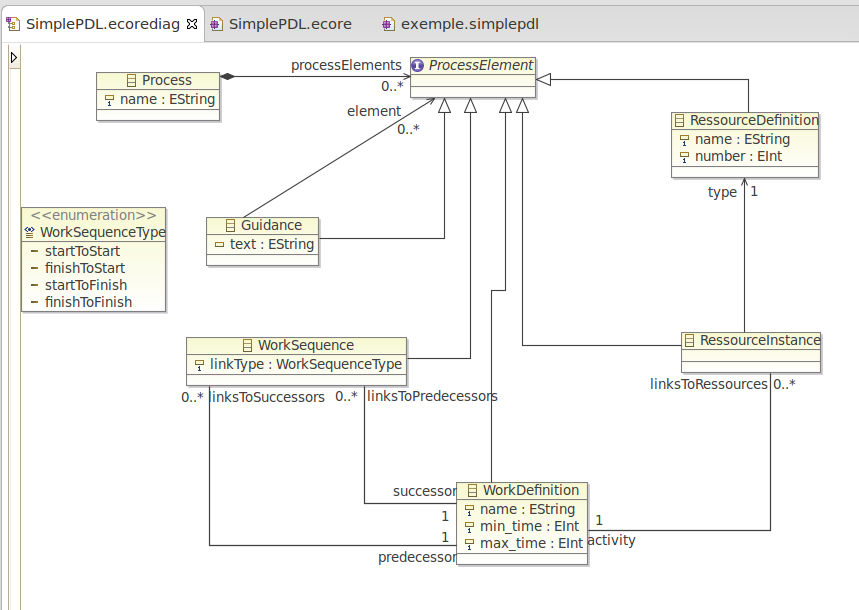
\includegraphics[width=15cm]{Capture-4.png}
\caption{Diagramme Ecore modifié} 
\label{img1} 
\end{center}
\end{figure} 

On se retrouve dans une situation assez symétrique avec les classes WorkDefinition et WorkSequence. En effet, ces deux classe héritent toutes deux de ProcessElement et une WorkSequence constitue un lien entre deux WorkDefinition.\\

Avec RessourceInstance et RessourceDefinition, une RessourceInstance consituera un lien entre une RessourceDefinition et une Activité.

\subsection{Ajout du temps}

L'ajout du temps est plus aisé (à ce niveau la en tout cas). Il suffit d'ajouter des attributs temps\_min et temps\_max aussi bien au niveau du Processus que de la WorkDefinition. Le fichier Ecore modifié est le suivant :\\

\begin{figure}[!h] 
\begin{center}
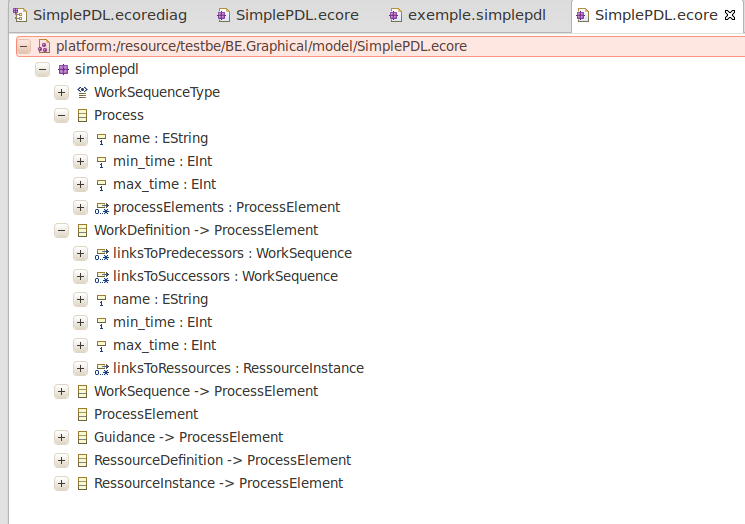
\includegraphics[width=10cm]{Capture-5.png}
\caption{Ecore avec gestion du temps} 
\label{img1} 
\end{center}
\end{figure} 

A présent que le fichier Ecore est mis à jour par rapport aux nouvelles spécifications, on va pouvoir modifier l'éditeur graphique GMF pour tenir compte des nouveautés ajoutées.

\newpage

\section{T2}

Il s'agit ici d'adapter l’éditeur graphique SimplePDL pour permettre de saisir graphiquement les ressources
disponibles et l’allocation des ressources nécessaires à chaque activité.

\ldots \ldots \ldots \ldots

\section{T3}

Nous devons donner une syntaxe concrète textuelle de SimplePDL pour prendre en compte les ressources
et le temps et l’outiller avec xText. On va donc reprendre la grammaire xText élaborée lors des séances précédentes.

On rajoute ces lignes dans le fichier xText :\\

\begin{verbatim}
RessourceDefinition returns RessourceDefinition:
	'rd'
		name=EString
		'number' number=EInt
	;

RessourceInstance returns RessourceInstance:
	'ri'
		'type' type=[RessourceDefinition|EString]
		'activity' activity=[WorkDefinition|EString]
		'instances' instances=EInt
	;
\end{verbatim}

On définit ainsi qu'une RessourceDefinition possède un nom et un chiffre indiquant sa quantité. Une RessourceInstance possède un type, qui n'est autre qu'une WorkDefinition.
Elle possède aussi une activité de type WorkDefinition et un nombre d'instances entier.\\

Il faut aussi modifier la ligne ProcessElement pour indique que RessourceDefinition et RessourceInstance en héritent.


\begin{verbatim}
ProcessElement returns ProcessElement:
	WorkDefinition | WorkSequence | Guidance | RessourceDefinition | RessourceInstance
	;
\end{verbatim}

Enfin, on ajoute au Processus et à la WorkDefinition des attributs min\_time et max\_time.

\begin{verbatim}
WorkDefinition returns WorkDefinition:
	'wd'
		name=EString
		'min' min_time=EInt
		'max' max_time=EInt
\end{verbatim}

et

\begin{verbatim}
Process returns Process:
	{Process}
	'process'
		name=EString
		'{'
			'min_time' min_time=EInt
			'max_time' max_time=EInt
			(processElements+=ProcessElement (processElements+=ProcessElement)* )?
		'}'
	;
\end{verbatim}

On peut à présent créer un fichier s'appuyant sur la grammaire crée.

\begin{verbatim}
process exemple {
	min_time 20
	max_time 50
	wd Conception min 10 max 16
	wd RedactionDoc min 8 max 12
	wd Development min 12 max 14
	wd RedactionTest min 10 max 12
	ws s2s from Conception to RedactionDoc
	ws f2f from Conception to RedactionDoc
	ws f2s from Conception to Development
	ws s2s from Conception to RedactionTest
	ws f2f from Development to RedactionTest
	rd concepteur number 3
	rd redacteur number 1
	rd developpeur number 2
	rd testeur number 2
	rd machine number 4
	ri type concepteur activity Conception instances 2
	ri type machine activity Conception instances 2
	ri type redacteur activity RedactionDoc instances 1
	ri type machine activity RedactionDoc instances 1
	ri type developpeur activity Development instances 2
	ri type machine activity Development instances 3
	ri type testeur activity RedactionTest instances 1
	ri type machine activity RedactionTest instances 2
}
\end{verbatim}

Ce fichier de modèle correspond à l'image suivante :\\

\begin{figure}[!h] 
\begin{center}
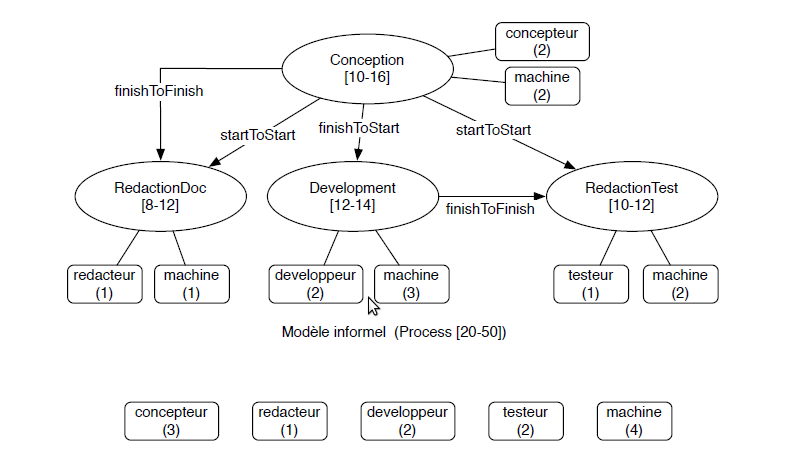
\includegraphics[width=15cm]{Capture-6.png}
\caption{Modèle utilisé dans le fichier dont la grammaire est définie par xText} 
\label{img1} 
\end{center}
\end{figure} 

\newpage

\section{T4}

On complète ici les contraintes OCL pour capturer les contraintes qui n’ont pu l’être par le métamodèle.

\subsection{Nom des ressources}

Comme pour les activités, il s'agit de vérifier que les ressources ont un nom unique.
On effectue donc un produit carthésien entre chaque Ressources.\\

\begin{verbatim}
-- Invariant vérifiant si toutes les ressources ont un nom unique
inv resourcesNamesAreDifferent:
	let elements : Set(ProcessElement) = self.processElements in
    	let rds: Set(ProcessElement) = elements->select(e | e.oclIsTypeOf(RessourceDefinition)) in
			rds->forAll(rd1, rd2: ProcessElement |
				if rd1 <> rd2 then
					rd1.oclAsType(RessourceDefinition).name <> rd2.oclAsType(RessourceDefinition).name
				else
					true
				endif
			)
\end{verbatim}

\subsection{Verification de la consistance}

On peut compléter la requète OCL des TPs, pour s'assurer que toutes les WorkDefinition associées à une RessourceInstance et les activités pointées par une WorkInstance appartiennent bien au même Processus.

\begin{verbatim}
inv containmentConsistency:
  let elements : Set(ProcessElement) = self.processElements in
    let wds: Set(ProcessElement) = elements->select( e | e.oclIsTypeOf(WorkDefinition)) in
      let wss: Set(ProcessElement) = elements->select( e | e.oclIsTypeOf(WorkSequence)) in
		let ris: Set(ProcessElement) = elements->select( e | e.oclIsTypeOf(RessourceInstance)) in
        -- WS linked to a process WD are elements of this process
        wds->forAll(wd: ProcessElement |
            elements->includesAll(wd.oclAsType(WorkDefinition).linksToPredecessors)
            and elements->includesAll(wd.oclAsType(WorkDefinition).linksToSuccessors)
			and elements->includesAll(wd.oclAsType(WorkDefinition).linksToRessources))
        -- source and target of a process WS are elements of this process
        and wss->forAll(ws: ProcessElement |
            elements->includes(ws.oclAsType(WorkSequence).predecessor)
            and elements->includes(ws.oclAsType(WorkSequence).successor))
		and ris->forAll(ws: ProcessElement |
            elements->includes(ws.oclAsType(RessourceInstance).type)
			and elements->includes(ws.oclAsType(RessourceInstance).activity))
\end{verbatim}

\subsection{Consistance des ressources}

On doit s'assurer qu'une WorkDefinition ne demande pas plus de ressources que le nombre maximal possible.
Par exemple, si on dispose de 4 machines au total et que la WorkDefinition conception en demande 6, le modèle n'est pas correct.

\begin{verbatim}
context RessourceInstance
inv ressourceCheck:
	if self.instances <= self.type.number then
		true
	else
		false
	endif
\end{verbatim}

\subsection{Vérification temporelle}

On doit s'assurer que la durée minimale d'une processus ou d'une WorkDefinition est bien inférieure à la durée maximale.

\begin{verbatim}
context WorkDefinition
inv timeCheck1:
	self.max_time < self.min_time implies
		false
\end{verbatim}

\section{T5}

Il faut à présent engendrer une nouvelle transformation SimplePdl to Petrinet. En effet, on doit reporter les changements réalisés dans méta-modèle SimplePdl, vers le méta-modèle PetriNet.\\

Nous allons de nouveau distinguer le cas des ressources de celui du temps.

\subsection{Ressources}

Pour les ressources, nous décidons de mettre en place le modèle suivant. Considérons deux types de ressources (RessourceDefinition), machine et testeur.
En admettant que une WorkDefintion (Conception dans cette exemple) nécéssite deux machines et un testeur, on aura le modèle suivant en pétri :\\

\begin{figure}[!h] 
\begin{center}
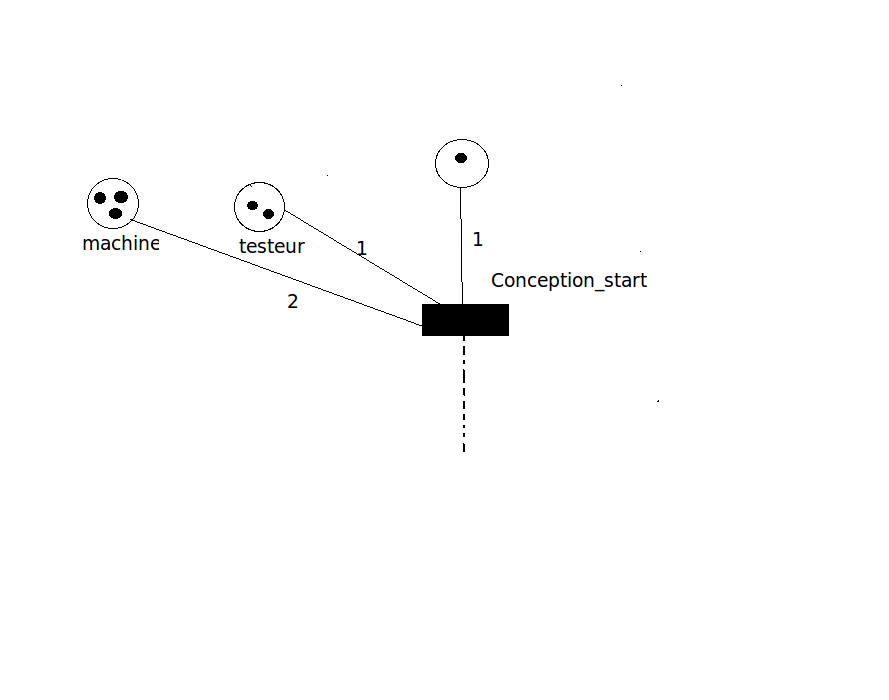
\includegraphics[width=10cm]{petri1.png}
\caption{Gestion des ressources} 
\label{img1} 
\end{center}
\end{figure} 

Basiquement on aura donc une règle permettant de parcourir les RessourceDefinition, qui seront traduites en places au sens des réseaux de pétri. L'attribut nombre de RessourceDefinition correspond directement au marquage de la place crée.

\begin{verbatim}
rule RessourceDefinition2PetriNet {
	from rd: simplepdl!RessourceDefinition
	to
		p_ressource: petrinet!Place(
						name <- rd.name,
						marking <- rd.number,
						net <- rd.getProcess())
}
\end{verbatim}

Il nous faut ensuite une règle qui pour chaque WorkInstance va créer un arc entre la place de la ressource et la transition de début de la WorkDefinition associée.
Il faut aussi crée un arc entre la transition de fin de la WorkDefinition et la place de la ressource. Cet arc traduit le fait que les ressources sont libérées à la fin de l'exécution de l'activité. Il est évident que l'on doit rendre autant de jetons que ceux qui ont été prélevés au démarrage de l'activité.

\begin{verbatim}
rule RessourceInstance2PetriNet {
	from ri: simplepdl!RessourceInstance
	to
		t_ressource_start: petrinet!Arc(
						source <- thisModule.resolveTemp(ri.type, 'p_ressource'),
						target <- thisModule.resolveTemp(ri.activity, 't_start'),
						weight <- ri.instances,
						kind <- #normal,
						net <- ri.getProcess()),
		t_ressource_finish: petrinet!Arc(
						source <- thisModule.resolveTemp(ri.activity, 't_finish'),
						target <- thisModule.resolveTemp(ri.type, 'p_ressource'),
						weight <- ri.instances,
						kind <- #normal,
						net <- ri.getProcess())
}
\end{verbatim}

\subsection{Temps}

Pour modéliser la gestion du temps dans un réseau de pétri, nous allons devoir mettre en place un observateur. Le principe de l'observateur est qu'il va nous fournir des informations sur le système sans pour autant en altérer le comportement. Typiquement, l'observateur d'une activité va nous informer sur le fait qu'elle se finit avec une durée correcte (comprise dans l'intervalle [temps\_min,temps\_max]), trop courte (durée exécution inférieure à la durée minimale) ou trop longue (durée exécution inférieure à la durée maximale).

\ldots \ldots 

TODO : METTRE PHOTO OBSERVATEUR POUR UNE SEULE ACTIVITE ET EXPLIQUER

Le code à fournir pour mettre en place cet observateur est assez long. Il n'est donc pas cité, mais est présent dans les rendus de ce BE.

\newpage

\section{T6}

L'étape de validation consiste à appliquer la transformation précédente et à l'appliquer à un exemple. Prenons le fichier de modèle suivant qui reprend l'exemple du sujet.

\begin{figure}[!h] 
\begin{center}
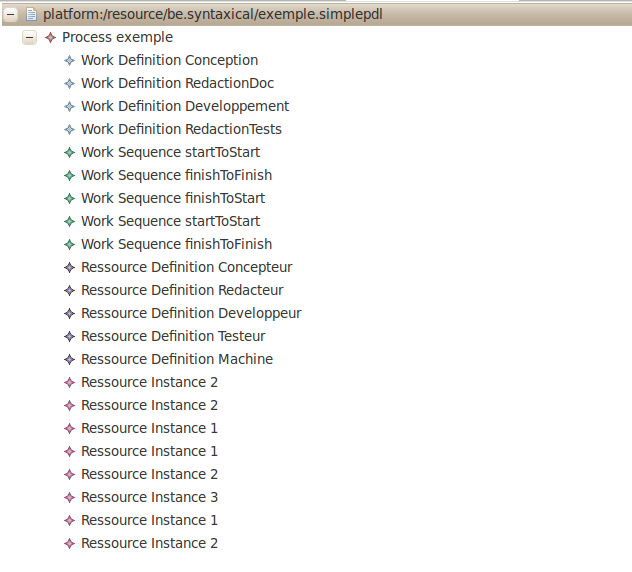
\includegraphics[width=10cm]{Capture-7.png}
\caption{Modèle SimplePDL conforme à l'exemple du sujet} 
\label{img1} 
\end{center}
\end{figure} 

Nous obtenons un fichier .PetriNet correspondant bien à ce qui était attendu. Il est valide par rapport au méta-modèle PetriNet.
On peut donc valider cette transformation et attaquer la partie PetriNet2Tina.

\section{T7}

Le méta-modèle PetriNet n'ayant pas évolué, il n'y a pas non plus de raisons de faire évoluer la transformation PetriNet2Tina. 
Nous avons juste du apporter quelques retouches par rapport à la version des TP. En effet, nous avions considéré que le temps associé par défaut à une transition est pas défaut
[0,0] sous tina. Pourtant, il s'agit d'un cas particulier puisque nous voulons que par défaut nos transitions soient de type [0,w[.\\

Dans cette transformation, on doit donc s'assurer que si temps\_max = -1 (signifie w car temps\_max forcément entier), alors le fichier de sortie comportera un intervalle terminé par w[.\\

\begin{verbatim}
-- build a Tina net file from a Petri net model
query PetriNet2Tina = 
	let repertoire: String = '/home/alex/workspace/BE/' in
		petrinet!PetriNet.allInstances()
			->collect(pn | pn.toTina().writeTo(repertoire + pn.name + '.net'));

-- concatenate all the strings of a sequence, adding the before char
-- before each string and the after char after.
helper
def: concatenateStrings(strings: Sequence(String),
		before: String, after: String): String =
	strings->iterate(s; acc: String = '' | acc + before + s + after);

-- translate a PetriNet element into the Tina textual syntax
helper 
context petrinet!PetriNet
def: toTina(): String =
	'net '  + self.name + '\n' + (
		let nodesStrings: Sequence(String) = self.nodes->collect(p | p.toTina())
		in
			thisModule.concatenateStrings(nodesStrings, '', '\n')
	)
;

-- translate a place to Tina syntax
helper
context petrinet!Place
def: toTina(): String =
	'pl ' + self.name + '(' + self.marking.toString() + ')'
;

-- translate a transition to Tina syntax.
helper
context petrinet!Transition
def: toTina(): String =
	let inNodesNames: Sequence(String)
		= self.incomings->collect(arc | arc.asTina(true))
	in let outNodesNames: Sequence(String)
		= self.outgoings->collect(arc | arc.asTina(false))
	in
		('tr '  + self.name
		+ ' [' + self.min_time + ',' + self.max_time + ']'
		+ thisModule.concatenateStrings(inNodesNames, ' ', '')
		+ ' -> '
		+ thisModule.concatenateStrings(outNodesNames, ' ', '')).regexReplaceAll('-1]', 'w[')
;
		
-- Translate an Arc to Tina syntax. isSource indicates if it is an
-- outgoing arc or an incoming one
helper
context petrinet!Arc
def: asTina(isSource: Boolean): String =
	if isSource = true then
		self.source.name
	else
		self.target.name
	endif
	+
	if self.kind = #normal then
		'*'
	else
		'?'
	endif
	+ self.weight.toString()
;
\end{verbatim}

\section{T8}
??

\section{T9}

Pour vérifier la terminaison d'un processus, il s'agit d'écrire plusieurs requètes LTL.
Soit l'opérateur finished qui correspond au ET logique entre toutes les places de fin de chaque activité, on a les propriétés suivantes :\\

[] (finished => dead);
Si l'on a fini, alors le réseau est mort, doit être Vrai.

[] <> dead;
Il est possible que le réseau soit mort, doit être Vrai.

[] (dead => finished);

- <> finished;


\section{T10}
TO BE DONE


\chapter{Partie 2}

Nous avons implémenté deux extensions supplémentaires qui apportent des fonctionnalités supplémentaires mais aussi de la compléxité au système. C'est pourquoi nous avons les avons implémenté en parallèle et façon à ce qu'elles soient indépendantes entre elles.

\section{Gestion plus fine des ressources}

Il s'agit dans cette extension de permettre qu'une activité en cours d'exécution puisse être interrompue puis reprendre le cours de son exécution. Une telle interruption doit libérer les ressources utilisées par l'activité en question qui deviennent alors disponibles pour une autre activité. Pour une activité interrompue, sa reprise doit être permise à condition que les ressources dont il dépend soient disponibles.\\
Pour cette extension, il n'est pas nécessaire de modifier la structure du méta-modèle SimplePDL, ce qui implique qu'il n'y a pas de modification à apporter à l'outil de génération de syntaxe concrète textuelle, ni à l'outil de syntaxe concrète graphique. En effet, on agira principalement sur le réseau de Petri résultant de la transformation à partir d'un modèle SimplePDL. Nous allons donc adapter la requête de transformation SimplePDL vers PetriNet afin de permettre l'interruption et la reprise (soumise à condition) d'une activité.

\subsection{Transformation SimplePDL vers PetriNet}

Il est nécessaire de modifier le réseau de Petri mais tout en veillant à toujours respecter la spécification stipulant qu'une activité est soit :
\begin{itemize}
\item non commencée - \textit{Ready}
\item en cours - \textit{Started}
\item terminée - \textit{Finished}
\end{itemize}
Il ne faut donc pas supprimer les états déjà mis en place dans la partie précédente.\\

D'autre part, il est préférable de ne pas altérer le fonctionnement général du réseau de Petri engendré par la requête conçue dans la première partie afin de ne pas risquer une regression au niveau des fonctionnalités, particulièrement au niveau des observateurs associés à chaque activité. C'est pourquoi nous avons fait le choix de rajouter des places représentant deux sous états de l'état \textit{Started} :
\begin{itemize}
\item en cours d'exécution - \textit{Running}
\item interrompue - \textit{Interrupted}
\end{itemize}
Deux nouvelles transitions sont nécessaire pour permettre à une activité d'osciller entre ces deux sous états :
\begin{itemize}
\item interrompre - \textit{Interrupt} : \textit{Running} vers \textit{Interrupted}
\item reprendre - \textit{Resume} : \textit{Interrupted} vers \textit{Running}
\end{itemize}
On remarque que ces nouveaux sous états ne changent rien au fonctionnement des observateurs mis en place dans la première partie, cela permet de répondre à l'exigence qui précise que quelque soit le sous état dans lequel on se trouve (\textit{Running} ou \textit{Interrupted}), le temps continue à être décompté.\\

Pour cela, il faut donc générer de nouvelles places représentant ces sous-états dans la requête de transformation SimplePDL vers PetriNet, pour tous les éléments \textit{wd} de type \textit{WorkDefinition} parcourus dans le modèle SimplePDL en entrée :
\begin{verbatim}
p_running: petrinet!Place(
        name <- wd.name + '_running',
        marking <- 0,
        net <- wd.getProcess()),
p_interrupted: petrinet!Place(
        name <- wd.name + '_interrupted',
        marking <- 0,
        net <- wd.getProcess()),
\end{verbatim}

Il faut également insérer les transitions, toujours depuis le contexte des éléments de type \textit{WorkDefinition} :
\begin{verbatim}
t_interrupt: petrinet!Transition(
        name <- wd.name + '_interrupt',
        incomings <- a_r2i,
        outgoings <- a_i2i,
        min_time <- 0,
        max_time <- -1,
        net <- wd.getProcess()),
t_resume: petrinet!Transition(
        name <- wd.name + '_resume',
        incomings <- a_i2r,
        outgoings <- a_r2r,
        min_time <- 0,
        max_time <- -1,
        net <- wd.getProcess()),
\end{verbatim}

De même pour les arcs :
\begin{verbatim}
a_r2i: petrinet!Arc(
        source <- p_running,
        target <- t_interrupt,
        weight <- 1,
        kind <- #normal,
        net <- wd.getProcess()),
a_i2i: petrinet!Arc(
        source <- t_interrupt,
        target <- p_interrupted,
        weight <- 1,
        kind <- #normal,
        net <- wd.getProcess()),
a_i2r: petrinet!Arc(
        source <- p_interrupted,
        target <- t_resume,
        weight <- 1,
        kind <- #normal,
        net <- wd.getProcess()),
a_r2r: petrinet!Arc(
        source <- t_resume,
        target <- p_running,
        weight <- 1,
        kind <- #normal,
        net <- wd.getProcess()),
\end{verbatim}

Les arcs suivants sont nécessaires pour la libération lors de l'interruption d'une activité et pour la prise de ressources lors de la reprise du cours de son exécution d'une activité. Dans ce cas-là, on se positionne depuis le contexte des éléments \textit{ri} de type \textit{RessourceInstance} qui font le lien entre une activité (\textit{WorkDefinition}) et un type de ressource (\textit{RessourceDefinition}) et qui contiennent la donnée du nombre de ressources requises (qui seront libérées et reprises successivement) :

\begin{verbatim}
a_i2r: petrinet!Arc(
        source <- thisModule.resolveTemp(ri.activity, 't_interrupt'),
        target <- thisModule.resolveTemp(ri.type, 'p_ressource'),
        weight <- ri.instances,
        kind <- #normal,
        net <- ri.getProcess()),
a_r2r: petrinet!Arc(
        source <- thisModule.resolveTemp(ri.type, 'p_ressource'),
        target <- thisModule.resolveTemp(ri.activity, 't_resume'),
        weight <- ri.instances,
        kind <- #normal,
net <- ri.getProcess())
\end{verbatim}

Afin de ne pas perturber le système de gestion des ressources initial, il est nécessaire de préciser quelques spécifications supplémentaires :
\begin{itemize}
\item Une activité qui entre dans l'état \textit{Started}, entre par défaut dans le sous-état \textit{Running}
\item Pour pouvoir traverser la transition \textit{Finish} amenant à l'état \textit{Finished}, il faut être dans le sous-état \textit{Running} et évidemment dans l'état \textit{Started}
\end{itemize}

Cela implique le rajout les arcs suivants :
\begin{verbatim}
a_s2r: petrinet!Arc(
        source <- t_start,
        target <- p_running,
        weight <- 1,
        kind <- #normal,
        net <- wd.getProcess()),
a_r2f: petrinet!Arc(
        source <- p_running,
        target <- t_finish,
        weight <- 1,
        kind <- #normal,
        net <- wd.getProcess()),
\end{verbatim}

\subsection{Exemple d'exécution}

Dans cet exemple d'exécution, on vérifie que :
\begin{itemize}
\item si on est dans le sous-état \textit{Running}, les ressources sont prises et que l'on peut accéder aux transitions \textit{Finish} et \textit{Interrupt}
\item si on est dans le sous-état \textit{Interrupted}, les ressources sont libérées et que l'on peut accéder à la transition \textit{Resume} et pas à la transition \textit{Finish}\\
\end{itemize}

On peut vérifier ces propriétés, avec une exécution en cinq phases sur une même activité, correspondant aux cinq états suivants, à l'aide du steppeur de l'outil Tina : 
\begin{itemize}
\item \textit{Ready}
\item \textit{Started} \textit{Running}
\item \textit{Started} \textit{Interrupted}
\item \textit{Started} \textit{Running}
\item \textit{Finihed}
\end{itemize}

\subsection{Contraintes LTL}

Afin de montrer que cette extension n'altère en rien les contraintes exiggées dans le document de spécification, on peut exécuter la requête LTL permetant de vérifier que si le processus est en \textit{Started}, alors toutes ses activités sont soit en \textit{Ready}, soit en \textit{Started}, soit en \textit{Finished}.

\section{Ressources alternatives}

Il s'agit ici de mettre en oeuvre une gestion alternative des ressources. Le principe est qu'il existe plusieurs configurations possibles de ressources.
Ainsi, soit une configuration A nécéssitant 2 machines et 3 développeurs et une configuration B avec 3 machines et 2 testeurs, on pourra exprimer le fait qu'une WorkDefition a besoin que la configuration A ou que la configuration B soit effective.

\subsection{Redéfinition du méta-modèle}

Il est donc clair que l'on doit modifier le méta-modèle pour expliciter cette possibilité de ``regroupement des ressources''.

\begin{figure}[!h] 
\begin{center}
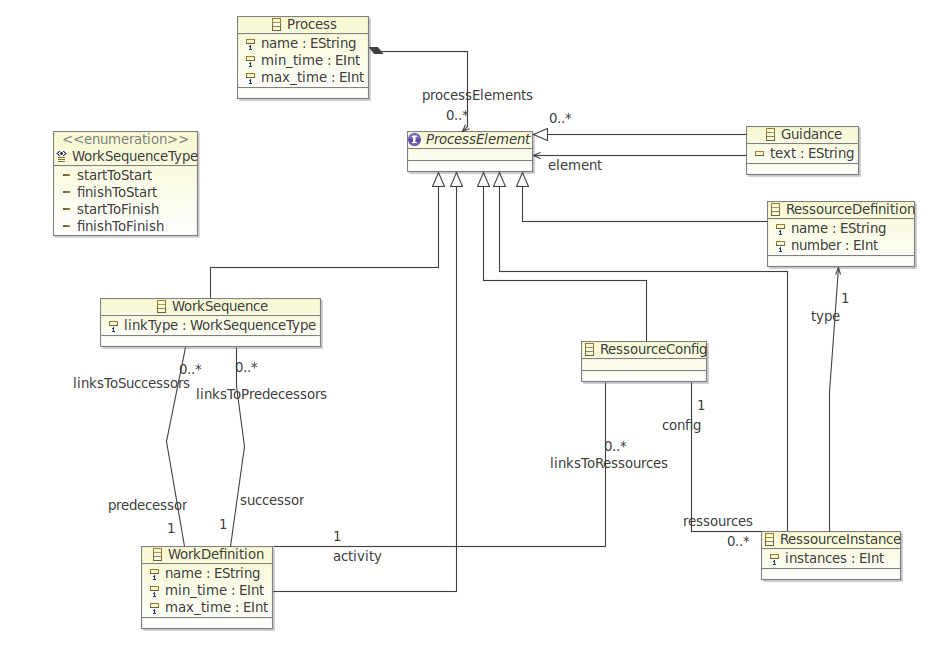
\includegraphics[width=15cm]{Capture-13.png}
\caption{Méta-modèle avec ressources alternatives} 
\label{img1} 
\end{center}
\end{figure} 

Et sous forme graphique,\\

\newpage

\begin{figure}[!h] 
\begin{center}
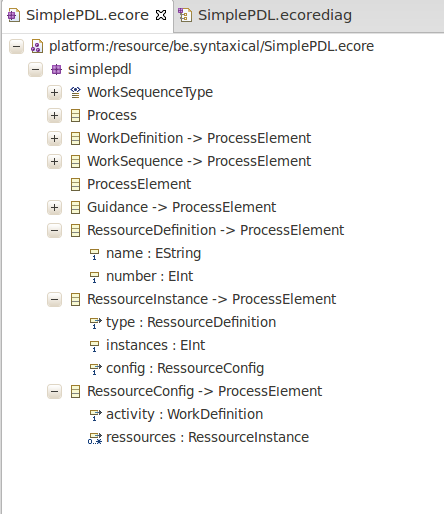
\includegraphics[width=8cm]{Capture-14.png}
\caption{Méta-modèle sous forme graphique} 
\label{img1} 
\end{center}
\end{figure} 

Pour permettre ce regroupement, on rajoute une classe RessourceConfig. Cette classe va contenir des liens vers des RessourceInstance. Ainsi, on va exprimer le fait qu'il peut exister plusieurs configurations mettant en oeuvre différents jeux de ressources.\\

On remplace donc le lien de WorkDefinition a RessourceInstance, par un lien de WorkDefinition a RessourceConfig. Ce lien a une multiplicité 0..\* car on peut avoir plusieurs Configurations pour une même WorkDefinition.

\subsection{Transformation SimplePDL vers PetriNet}

Prenons l'exemple suivant, 

\begin{figure}[!h] 
\begin{center}
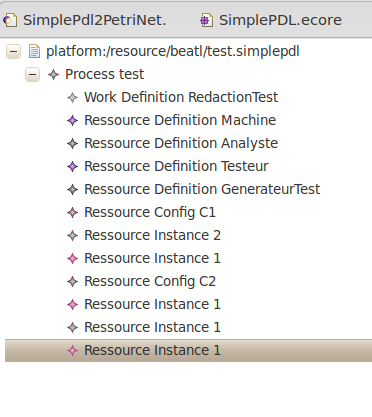
\includegraphics[width=8cm]{Capture-15.png}
\caption{Exemple mis en oeuvre} 
\label{img1} 
\end{center}
\end{figure}

On dispose de 4 ressources : Machine, Analyste, Testeur, GenerateurTest.
Par souci de lisibilité, on limite le nombre de WorkDefinition, à une seule : redactionTest. On définit également deux configurations C1 et C2. C1 met en oeuvre deux WorkInstance (Machine, 2) et (GenerateurTest,1). C2 met en oeuvre trois WorkInstance (Analyste,1), (GenerateurTest,1) et (Machine,1).\\

Cet exemple va nous permettre d'illustrer les transformations qui doivent être effectuées.\\

Il faut donc reprendre la transformation SimplePDL vers PetriNet et transformer la gestion des Ressources. Toujours par souci de lisibilité, on s'affranchit de la génération d'observateurs.\\

Le principe du réseau de pétri gérant la configuration des ressources est le suivant :\\

\begin{itemize}
\item Il est possible de choisir entre chacune des configurations (si du moins il y a suffisament de ressources)
\item Une fois que l'on a choisi de démarrer avec une configuratio, on ne pourra plus choisir l'autre
\item Les Ressources utilisées doivent être restituées à la fin de l'activité, et qui plus est dans la bonne configuration.
\end{itemize}

Il ressort de cette analyse que l'on va devoir utiliser des places nous indiquant :\\

\begin{itemize}
\item Quelle configuration est choisie : ConfigurationName\_used
\item Une configuration a été choisie : ProcessName\_ress\_l\\
\end{itemize}

Et des transitions pour :\\

\begin{itemize}
\item Choisir une configuration : ConfigurationName.start
\item Rendre les ressources : ConfigurationName.finished\\
\end{itemize}

Pour l'exemple cité précédement, on obtient donc le réseau de pétri suivant :\\

\begin{figure}[!h] 
\begin{center}
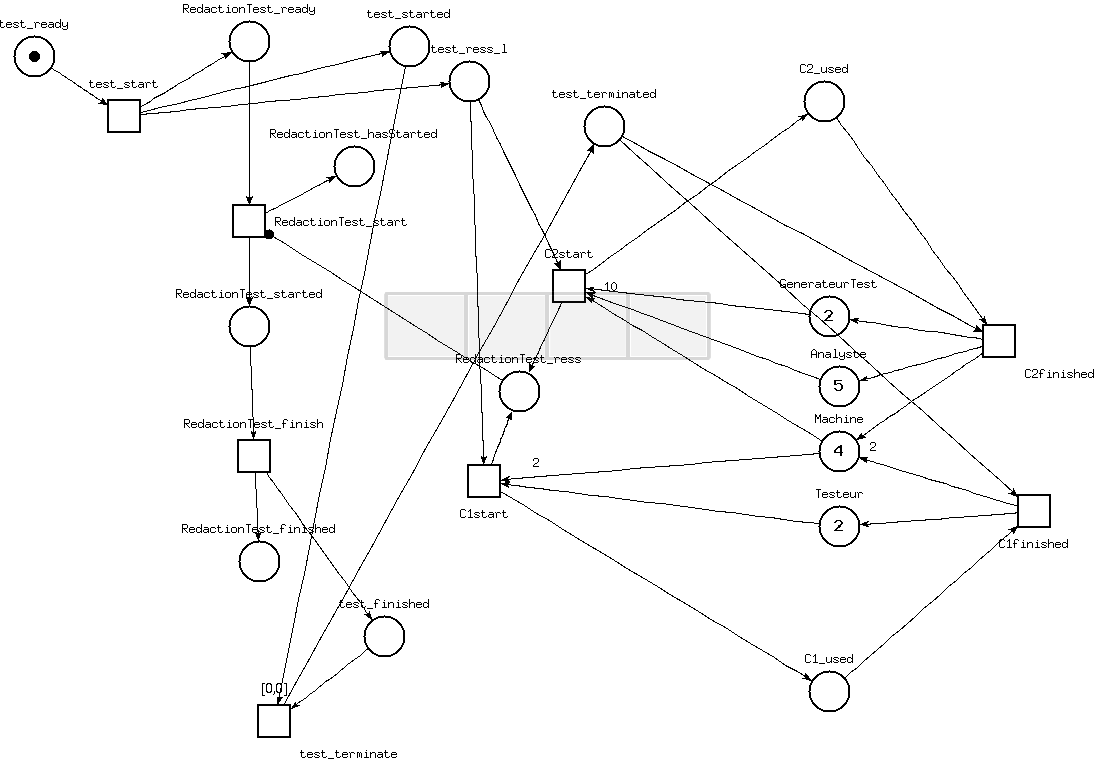
\includegraphics[width=15cm]{Capture-16.png}
\caption{Réseau de pétri obtenu} 
\label{img1} 
\end{center}
\end{figure}

Bien entendu, le code de la transformation a été adapté pour fornir ces changements. Il est disponible en annexe.\\

Pour ce qui est de la transformation PetriNet2Tina, il n'y a toujours aucune raison de la modifier car, on a pu conserver la même structure pour le méta-modèle PetriNet.ecore.\\








\end{document}   
